\appendix
\section{Derivation of the branch decomposition
(Eq.~\ref{eq:branches})}
\label{app:branches}

Fix a query (image, caption), a $\sigma$, and an arm $a$. Per draw
$\epsilon$, the adapter gradient of the $\tfrac12$-scaled loss is the
product $g_a(\epsilon) = J_a(\epsilon)^{\!\top} r_a(\epsilon)$ of
\S\ref{sec:branches}. Split each factor into its noise mean and
fluctuation, $J_a = \bar J_a + \tilde J_a$ and
$r_a = \bar r_a + \tilde r_a$ with
$\mathbb{E}_\epsilon[\tilde J_a] = 0$ and
$\mathbb{E}_\epsilon[\tilde r_a] = 0$; the population mean gradient of
arm $a$ is then
\begin{equation}
\bar g_a \;=\; \mathbb{E}_\epsilon\!\big[J_a^{\!\top} r_a\big]
\;=\; \bar J_a^{\!\top} \bar r_a
\;+\; \mathbb{E}_\epsilon\!\big[\tilde J_a^{\!\top} \tilde r_a\big].
\label{eq:appmean}
\end{equation}
Write the demoted arm's mean factors as native plus a perturbation,
$\bar J_e = \bar J + \Delta J$ and $\bar r_e = \bar r + \Delta \bar r$
(bars without an arm subscript denote the native arm). Subtracting
Eq.~\ref{eq:appmean} across arms and expanding the product,
\begin{equation}
\delta g \;=\; \bar g_e - \bar g_{\mathrm{nat}}
\;=\;
\underbrace{\bar J^{\!\top} \Delta\bar r}_{B_e}
\;+\;
\underbrace{\Delta J^{\!\top}\, \bar r}_{C_e}
\;+\;
\underbrace{\Delta J^{\!\top} \Delta\bar r
\;+\;
\mathbb{E}_\epsilon\!\big[\tilde J_e^{\!\top}\tilde r_e\big]
- \mathbb{E}_\epsilon\!\big[\tilde J_{\mathrm{nat}}^{\!\top}
\tilde r_{\mathrm{nat}}\big]}_{R_e}.
\label{eq:appbranches}
\end{equation}
This is an exact identity --- no linearization is involved.
``First-order'' in the main text refers only to the content of $R_e$:
it collects every term that is a product of two perturbations
($\Delta J^{\!\top} \Delta\bar r$) or a difference of noise-covariance
terms (the last two). Eq.~\ref{eq:branches} is
Eq.~\ref{eq:appbranches} with the mean-Jacobian bar suppressed in the
notation.

One remark delimits the identity's literal scope, expanding the
qualification stated in \S\ref{sec:branches}. When the two arms share
a grid (as for the re-encoding control), every operation above is
literal. Across grids, $J_{\mathrm{nat}}$ and $J_e$ act on different
token counts, so the differences $\Delta J$ and $\Delta \bar r$ require
a fixed identification of the two output spaces (e.g.\ spectral
zero-padding of the coarse grid onto the fine grid's bands); any such
identification changes the split between $B_e$, $C_e$, and $R_e$ but
not their sum $\delta g$, which lives in the shared adapter-parameter
space regardless. This is why the main text defines the branches
\emph{operationally} --- as the two independent perturbation directions
in adapter-parameter space, isolated by the designated probes of
\S\ref{sec:floor} --- and treats Eq.~\ref{eq:branches} as fixing what
each branch collects rather than as a computable matrix formula.

\section{Derivation of the angular forms (Eqs.~\ref{eq:exact}
and~\ref{eq:fourterm})}
\label{app:geometry}

Both angular forms follow from Eq.~\ref{eq:gapdef} and the split of
$\delta g$ by the native direction; no property of demotion enters.
Write $g = \bar g_{\mathrm{nat}}$, $G = \|g\|$, $\hat g = g/G$, and
decompose
$\delta g = G\,\kappa_\parallel\, \hat g + P_{\!\perp}\delta g$ with
$\kappa_\parallel = \hat g^{\!\top}\delta g / G$ and
$\kappa_\perp = \|P_{\!\perp}\delta g\| / G$.

\paragraph{The exact form.} The two components are orthogonal, so
$\|g + \delta g\|^2 = G^2 (1+\kappa_\parallel)^2 + G^2 \kappa_\perp^2$
and
\begin{equation}
\cos\big(g,\, g + \delta g\big)
\;=\; \frac{\hat g^{\!\top}(g + \delta g)}{\|g + \delta g\|}
\;=\; \frac{1 + \kappa_\parallel}
{\sqrt{(1+\kappa_\parallel)^2 + \kappa_\perp^2}}
\;=\; \frac{1}{\sqrt{1 + \kappa_{\mathrm{eff}}^2}}\,,
\qquad
\kappa_{\mathrm{eff}} = \frac{\kappa_\perp}{1 + \kappa_\parallel}\,,
\label{eq:appexact}
\end{equation}
valid whenever $1 + \kappa_\parallel > 0$ (the perturbation does not
reverse the gradient direction); $d_e = 1 - \cos$ is
Eq.~\ref{eq:exact}. Since
$1 - \cos(\hat g_1, \hat g_2) = \tfrac12 \|\hat g_1 - \hat g_2\|^2$
for unit vectors, starting from either expression in
Eq.~\ref{eq:gapdef} lands on the same result.

\paragraph{The quadratic limit.} For small perturbations,
$1 - (1 + \kappa_{\mathrm{eff}}^2)^{-1/2}
= \tfrac12 \kappa_{\mathrm{eff}}^2 + O(\kappa_{\mathrm{eff}}^4)$ and
$\kappa_{\mathrm{eff}}^2 = \kappa_\perp^2\big(1 - 2\kappa_\parallel
+ O(\kappa_\parallel^2)\big)$, so
\begin{equation}
d_e \;=\; \frac{\|P_{\!\perp}\delta g\|^2}{2 G^2}
\;+\; \underbrace{O(\kappa_\perp^2 \kappa_\parallel)
+ O(\kappa_\perp^4)}_{\text{beyond-quadratic}}.
\label{eq:appquad}
\end{equation}

\paragraph{The four-term expansion.} Substituting
$\delta g = B_e + C_e + R_e$ (Eq.~\ref{eq:branches}) into the leading
term and expanding the square,
\begin{equation*}
\|P_{\!\perp}\delta g\|^2
= \|P_{\!\perp}B_e\|^2 + \|P_{\!\perp}C_e\|^2
+ 2\,\langle P_{\!\perp}B_e,\, P_{\!\perp}C_e\rangle
+ \Big(2\,\langle P_{\!\perp}(B_e{+}C_e),\, P_{\!\perp}R_e\rangle
+ \|P_{\!\perp}R_e\|^2\Big),
\end{equation*}
whose first three terms, divided by $2G^2$, are exactly the data
share $S_e$, the graph share $F_e$, and the projected interaction
$I_e$ of Eq.~\ref{eq:fourterm}. The remainder $R'_e$ of
Eq.~\ref{eq:fourterm} therefore has an exact content: the
$R_e$-bearing terms above, the beyond-quadratic terms of
Eq.~\ref{eq:appquad}, and the parallel-component correction --- each
suppressed by an extra power of perturbation size relative to the
retained terms.

\paragraph{What is not derived.} The loading
$\|P_{\!\perp}\delta g\| = c_e\, m(\sigma)$ --- that the orthogonal
gradient mismatch is proportional to the residual mismatch with a
$\sigma$-independent route gain --- is an empirical ingredient
(the data-branch factorization at the amplitude level), fit and tested
held-out in
\S\ref{sec:confronted}. The geometry above fixes only how a given
$\delta g$ is read into gap units.

\section{Instrument details}
\label{app:instrument}

\paragraph{Estimator.} Per image, arm, and $\sigma$-bin, adapter gradients
are accumulated over $D$ stratified draws and flattened; cosines are taken
between accumulated vectors. Per-bin cosines at $D{=}8$ are not comparable
\emph{across} bins (the floor drops where $\|g\|$ is small); the gap
subtraction against the same-bin floor is the valid read. Split-half
reliability over images of each bin-mean curve is mandatory
(observed $0.73$--$0.88$ on verdict runs); a per-image variant of the same
quantity has split-half reliability ${\approx}\,0$ and is never used.

\paragraph{Controls.} The re-encoding arm prices the VAE decode--encode
round trip that demotion necessarily pays; in pre-debiasing runs its gap
served as the validity band ($\pm 0.04$; observed $|\cdot| \le 0.054$
across all bins of the main runs, per-module-group $\le 0.045$ in the
split runs), a role superseded by the paired debiased read of
\S\ref{sec:instrument}. The redraw floor prices finite-draw noise.
Density-weighting the uniform bins by the trainer's $\sigma$-density
reproduces earlier $\sigma$-marginalized measurements from the same
instrument family (consistency check).

\paragraph{Debiasing (\S\ref{sec:debias}), implementation.} Under
\texttt{--self\_floor}, every arm (re-encoding and each demote variant)
runs a second independent draw set from a disjoint seed stream, giving
per-arm self-cosines alongside the native floor; Eq.~\ref{eq:debias} is
then computed per image and bin, and the map read is the paired
excess $\Delta_i = \dgap_{e,i} - \dgap_{\reenc,i}$ with non-finite
values (negative self-cosines under the square root at low $D$) and
$|\Delta_i| > 1.5$ trimmed ($0$--$5$ of $40$ images per cell). Under
\texttt{--draw\_sweep}, draw prefixes are nested ($D = 64$ contains the
$D \le 32$ sets; prefix sums, no extra forwards) and
$\gap(D) = \gap_\infty + c/D$ is fit on route means with a bootstrap CI
over images. Finite-draw cosines are kernel-path chaotic: twin runs
sharing a warm compiler kernel cache agree to $|\Delta\cos| \le 0.015$,
while a run compiled to a different kernel set lands up to
${\approx}\,0.3$ away at $D{=}2$ --- so gap/floor/self-floor pairings
are never compared across processes, a guarantee the single-run
instrument provides by construction; a \texttt{--deterministic} mode
(bit-exact across twin runs) covers the paired training A/Bs.

\paragraph{Endpoint and x-zero modes.} The $\sigma{=}1$ endpoint bin feeds
input exactly $\epsilon$ (the input-mediated data term vanishes by
construction). The x-zero mode zeroes $x$ in input \emph{and} target on
every grid, keeping captions and exact demoted latent shapes; with the
$(1{-}\sigma)x$ term absent, low-$\sigma$ bins are off-manifold and the
$\sigma{=}1$ read is primary. In that regime the residual is
${\approx}\,{-}\hat x_{\mathrm{prior}}$, so ``graph-dominated'' includes
the model's grid-conditioned prior; the prior-distance probe
(\S\ref{sec:floor}) subsequently dissociated the prior from the floor's
route ordering.

\begin{figure}[t]
\centering
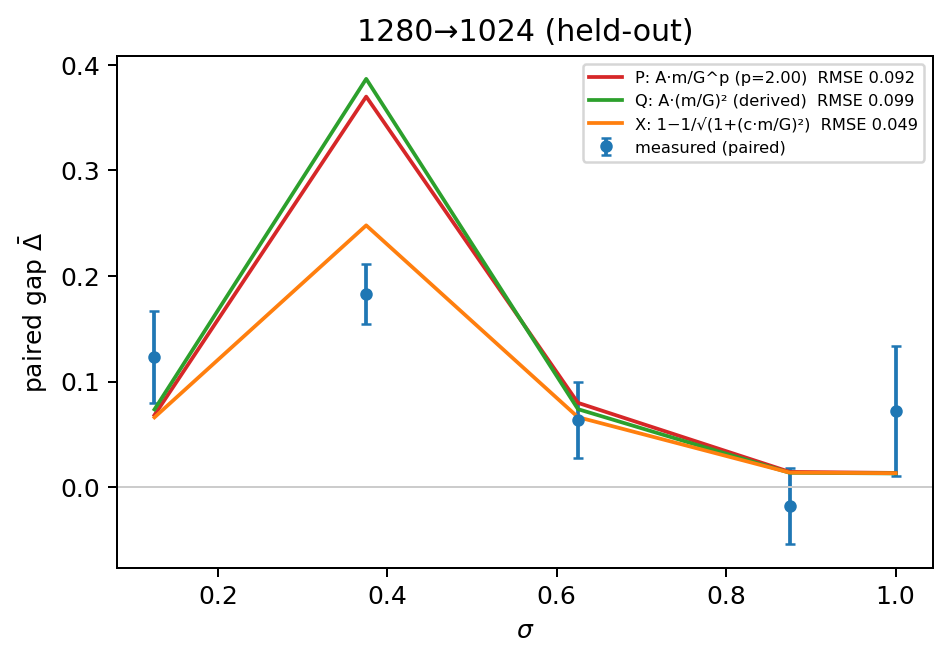
\includegraphics[width=0.55\linewidth]{figs/e5_refit_1280.png}
\caption{The second held-out route, $1280{\to}1024$, under the same
three functional forms as Fig.~\ref{fig:e5} --- predicted from
governors fitted on other routes. The derived quadratic systematically
overshoots the mid-$\sigma$ peak; the exact angular link's saturation
removes the overshoot (RMSE $0.049$ vs ${\approx}\,0.095$,
\S\ref{sec:confronted}).}
\label{fig:e51280}
\end{figure}

\paragraph{Held-out validation and refit (\S\ref{sec:confronted}),
sources.} The fit consumes the debiased paired curves of the
$1024$-tier verdict run, the $1280$-tier curves (pre-debiasing paired
reads; caveat recorded in \S\ref{sec:limitations}), the route-uniform
$m(\sigma)$ from the residual probe, and each run's own bin-mean
$G(\sigma)$ (gap and $G$ always from the same process, per the
kernel-path rule). The shared-power fit scans $p \in [1, 2]$ jointly
across fit routes with per-route weighted least squares; the exact-link
fit is a per-route grid with profile-likelihood uncertainties on $c_e$.
Oracle baselines are quadratic-in-$\sigma$ fits on the held-out data
itself (the noise ceiling for a 3-dof curve); the null baseline is
gap $= 0$ on the null's committed region $\sigma > \sigma_{\mathrm{eq}}$.

\paragraph{Spectral-null computation.} Table~\ref{tab:null} evaluates
Eq.~\ref{eq:spd} at the demoted grids' Nyquist frequencies
$f_{\mathrm{cut}} = \tfrac{1}{2}\,e/e_{\mathrm{nat}}$ on the $N{=}40$
mean radially-averaged latent power spectrum ($64$ radial bins; $P$ at
the $896/768/512$ cuts $= 0.025/0.029/0.065$). The equal-power slice
$\delta = (1+P_\omega)/2$ recovers
$\sigma_{\mathrm{eq}} = \sqrt{P}/(1+\sqrt{P})$ exactly. Across
$\delta \in [0.001, 0.5]$ the mildest--harshest spread never exceeds
$0.13$, and the $1024{\to}896$ versus $896{\to}768$ boundaries (cut
frequencies $0.4375$ vs $0.4286$) never separate by more than $0.01$.
The parameter-free anchor $\delta_{\reenc}$ of \S\ref{sec:phenomenon} is
measured by the same estimator: RAPSD of the re-encode arm's latent error
(fresh resize--encode minus cached latent, the gradient probe's own
control chain) on the same probe set, interpolated at each route's cut
frequency. Measured ($N{=}40$, $64$ radial bins): error variance
$2.7\times10^{-5}$ against latent variance $0.419$;
$D(f_{\mathrm{cut}}) \approx 1.0\times10^{-5}$ at all three cuts
(p10--p90 over images within $[1, 2]\times10^{-5}$), giving
$t^{*}_{\reenc} = 0.98 / 0.98 / 0.99$ for $896/768/512$.

\section{Controlled-adapter replication of the verdict map}
\label{app:e7}

\begin{figure}[t]
\centering
\begin{subfigure}[t]{0.49\textwidth}
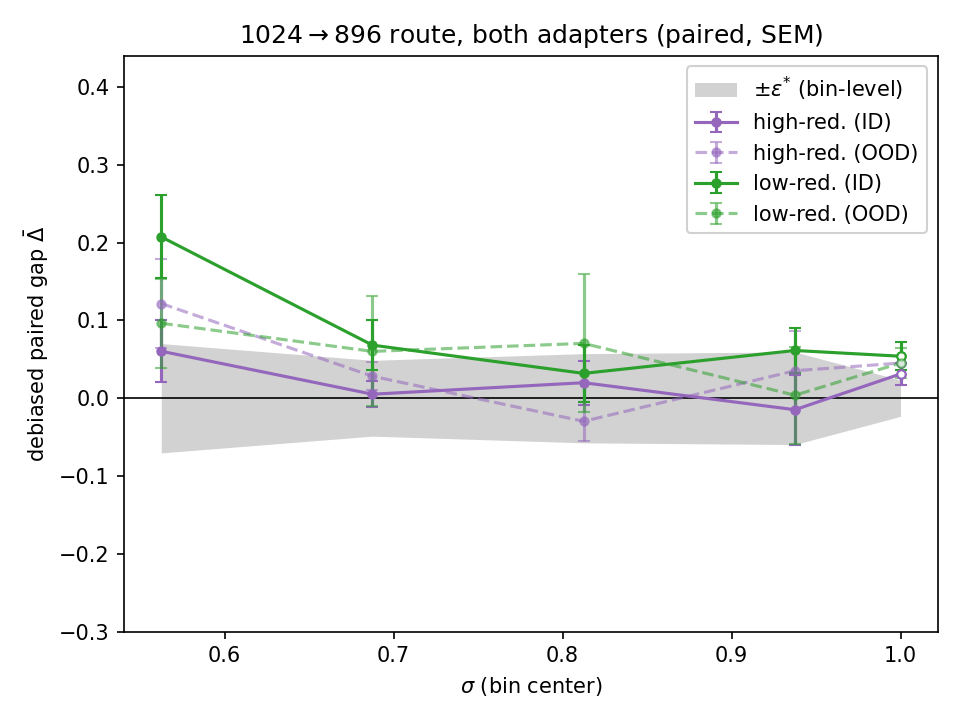
\includegraphics[width=\linewidth]{figs/gap_debiased_e7_route896.png}
\caption{$1024{\to}896$ (the certified route).}
\label{fig:e7route896}
\end{subfigure}\hfill
\begin{subfigure}[t]{0.49\textwidth}
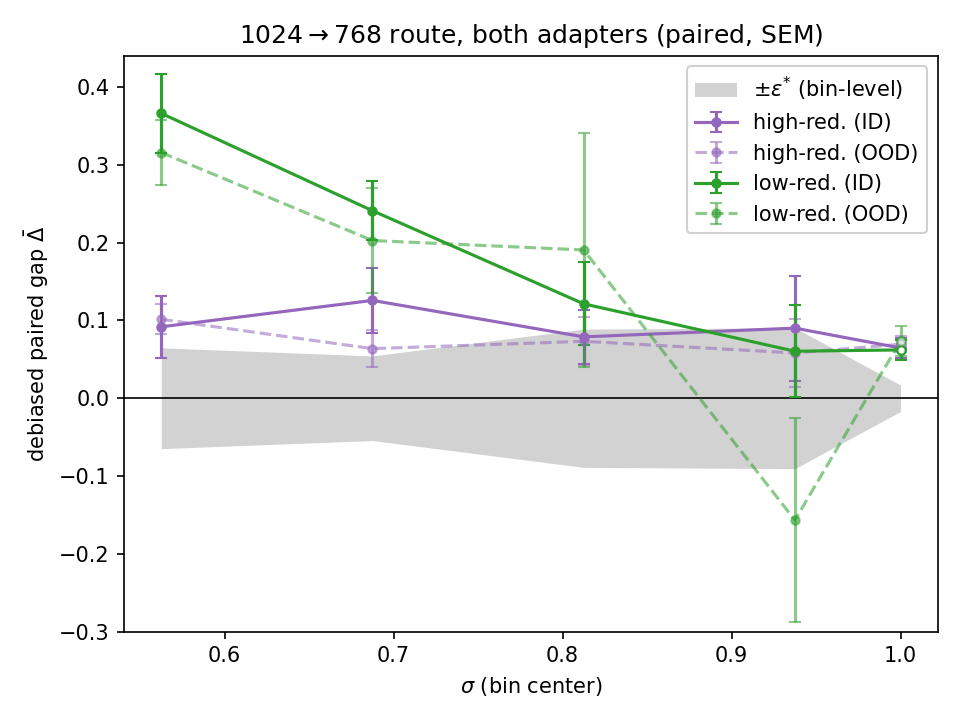
\includegraphics[width=\linewidth]{figs/gap_debiased_e7_route768.png}
\caption{$1024{\to}768$.}
\label{fig:e7route768}
\end{subfigure}
\caption{The Fig.~\ref{fig:gapcurves} recipe repeated on two controlled
adapters trained on opposite style clusters, one panel per route
($N{=}48$ stems per adapter, $D{=}8$/bin, high-$\sigma$ window; same
paired debiased estimator and trim; open markers the $\sigma{=}1$
endpoint bin; axes shared across panels). Unlike the main-text figures,
color encodes the \emph{adapter} (high- vs low-redundancy cluster);
solid curves are in-distribution stems --- the adapter's own style
cluster ($n{=}36$: trained-on, held-out, and never-seen-artist cells)
--- and dashed curves are out-of-distribution stems from the opposite
cluster ($n{=}12$). Gray band: bin-level $\pm\epsstar$ per
Eq.~\ref{eq:safe}, median of the two runs' full-$N$ SEMs for the
panel's route. The map replicates: on the certified route all four
adapter$\times$distribution curves reach the band inside the window,
on $768$ all four sit above it until the top, and within each panel the
dashed OOD curves track their solid ID counterparts --- the
adapter$\times$probe-style interaction is not visible at this
resolution.}
\label{fig:e7maps}
\end{figure}

The one-adapter caveat of \S\ref{sec:limitations} pre-registered a
controlled $2{\times}2$ factorial: two plain-LoRA checkpoints trained
under the shipped probe adapter's frozen recipe on opposite style
clusters --- the top and bottom $12$ artists by median latent
redundancy, hereafter the high-redundancy (visually flat) and
low-redundancy (heavily textured) clusters --- with stem-level
membership manifests frozen
before training ($124$ training images each, identical seeds). Each
adapter was probed on $48$ stems spanning four membership cells
($N{=}12$ each): trained-on, held-out images of trained artists,
never-seen artists of the same cluster, and never-seen artists of the
opposite cluster, with the cross-cluster stems shared between the two
runs so cross-adapter contrasts read paired per stem.
Figure~\ref{fig:e7maps} repeats the verdict-map recipe per route,
overlaying both adapters.

Three reads, stated at the bin-mean level (per-cell tables reproduce
from the archived per-image rows). First, the $(\text{route}, \sigma)$
shape replicates on both checkpoints (Fig.~\ref{fig:e7maps}). Second,
the factorial contrasts are null at instrument resolution: the
probe-style main effect and the adapter$\times$probe-style interaction
--- the pre-registered verdict quantity --- are both bounded below the
resolvable bin-mean effect (raw-gap paired interaction
$-0.022 \pm 0.027$ at $896$, $-0.015 \pm 0.059$ at $768$), and the
membership contrast (trained-on versus held-out) does not replicate in
sign across the two adapters. The map is therefore adapter- and
content-agnostic on this model at our resolution, supporting the
calibrate-once-per-model reading of \S\ref{sec:map}. Third, the one
quantity that is \emph{not} checkpoint-invariant is the absolute
redraw-floor level: in-window floor cosines sit at ${\approx}0.73$ for
the high-redundancy-cluster adapter versus ${\approx}0.50$ for the
low-redundancy-cluster adapter, uniformly across all four membership
cells including the opposite-cluster stems. The floor's level is a property of the
checkpoint (its gradient stochasticity), while the safety map built on
top of it is not.

\section{Historical (pre-debiasing) tables}
\label{app:tables}

The tables in this appendix are the raw-estimator record: retained for
continuity and for the reads defended in \S\ref{sec:instrument}
(one-signed bias; paired same-grid contrasts), never cited as debiased
evidence.

\begin{table}[h]
\caption{\textbf{Raw estimator} (historical record; superseded by
Table~\ref{tab:debiasedmap}): demotion gap by
$\sigma$-bin, $1024$-tier natives ($N{=}40$,
bin-mean SEM ${\sim}0.02$, re-encoding control $|\gap_\reenc| \le 0.054$
everywhere, split-half reliability $0.73$--$0.83$). Bold = within the
re-encoding band. Raw values understate mid-$\sigma$ gaps (the floor
attenuates the read) and overstate endpoint floors (single-estimate
variance bias); the debiased map corrects both. The $\cos_{\mathrm{floor}}$
and $\|g\|$ rows are the estimator context plotted in
Fig.~\ref{fig:estimator}.}
\label{tab:phase0}
\centering
\small
\begin{tabular}{lcccccccc}
\toprule
$\sigma$ bin center & 0.06 & 0.19 & 0.31 & 0.44 & 0.56 & 0.69 & 0.81 & 0.94 \\
\midrule
$\gap_{896}$ (ratio $0.875$) & .110 & .162 & .148 & .137 & \textbf{.048} & \textbf{.030} & \textbf{.030} & .053 \\
$\gap_{768}$ (ratio $0.75$)  & .144 & .216 & .208 & .223 & .164 & .163 & .115 & .063 \\
$\gap_{512}$ (ratio $0.5$)   & .348 & .410 & .355 & .469 & .430 & .391 & .289 & .296 \\
\midrule
$\cos_{\mathrm{floor}}$ & .84 & .65 & .51 & .65 & .70 & .77 & .80 & .83 \\
$\|g\|$ (native) & 2.6 & 0.5 & 0.4 & 0.5 & 0.7 & 1.1 & 2.0 & 9.3 \\
\bottomrule
\end{tabular}
\end{table}

\begin{table}[h]
\caption{Raw endpoint reads ($D{=}16$, $N{=}40$) beside their debiased
draw-limit values (Table~\ref{tab:floor}) --- the debiasing's revision
record: the $768$ floor halves, the $896$ floor surfaces.}
\label{tab:rawendpoint}
\centering
\small
\begin{tabular}{lcc}
\toprule
route & raw endpoint ($D{=}16$) & endpoint $\dgap_\infty$ [95\% CI] \\
\midrule
native self-floor (cosine) & $0.85$ & $1.005$ $[0.994, 1.016]$ \\
re-encoding control & $-0.038$ & $-0.003$ $[-0.017, +0.008]$ \\
$1024{\to}896$ & $-0.009$ & $+0.019$ $[+0.010, +0.030]$ \\
$1024{\to}768$ & $+0.127$ & $+0.056$ $[+0.043, +0.071]$ \\
$1024{\to}512$ & $+0.326$ & $+0.304$ $[+0.197, +0.424]$ \\
\bottomrule
\end{tabular}
\end{table}

\begin{table}[h]
\caption{Iso-severity probe (\textbf{raw estimator}): gap by $\sigma$-bin
on the $1280$-tier cache
($N{=}24$, $4$ draws/bin) against the corpus $1024{\to}896$ curve. The
ratio-matched routes coincide within ${\sim}1.4$ combined SEM at every bin
despite a $1.6\times$ difference in absolute target size; the same-native
harsher-ratio route separates. $^{*}$$896$'s canonical $16$-draw endpoint
is $-0.009$ raw, $+0.019$ debiased (Table~\ref{tab:floor}).}
\label{tab:isoseverity}
\centering
\small
\begin{tabular}{lccccc}
\toprule
$\sigma$ & 0.125 & 0.375 & 0.625 & 0.875 & 1.0 \\
\midrule
re-encoding control & $+.047$ & $-.005$ & $+.048$ & $+.020$ & $-.012$ \\
$1280{\to}1120$ (ratio $.875$) & .129 & .110 & .054 & $-.012$ & $-.007$ \\
$1280{\to}1024$ (ratio $.80$)  & .170 & .178 & .111 & .002 & .061 \\
$1024{\to}896$ (ratio $.875$)  & .132 & .076 & .077 & .049 & .100$^{*}$ \\
\bottomrule
\end{tabular}
\end{table}

\begin{table}[h]
\caption{Ratio-transfer run (\textbf{raw estimator}): $896$-tier natives
($N{=}40$), pre-registered
bar ``$\gap_{768}$ within the re-encoding band at $\sigma \ge 0.5$'' ---
\textbf{fails} (residual $0.06$--$0.12$, ${\sim}2\times$ the
$1024{\to}896$ plateau; ${\sim}$half of it is expected estimator bias,
\S\ref{sec:instrument} --- the separation is independently confirmed by
the debiased same-grid floors, \S\ref{sec:floor}).}
\label{tab:phase1a}
\centering
\small
\begin{tabular}{lcccccccc}
\toprule
$\sigma$ bin & 0.06 & 0.19 & 0.31 & 0.44 & 0.56 & 0.69 & 0.81 & 0.94 \\
\midrule
$896{\to}768$ & .114 & .209 & .168 & .143 & .124 & .056 & .092 & .061 \\
$896{\to}512$ & .318 & .372 & .308 & .340 & .320 & .280 & .329 & .217 \\
\bottomrule
\end{tabular}
\end{table}

\begin{table}[h]
\caption{Route-uniformity of the mean prediction residual: cross-grid
excess of $\bar r = \mathbb{E}_\epsilon[\hat v - (\epsilon - x)]$ over
split-half floors (relative $L_2$; same-grid re-encoding control
$\le 0.02$ everywhere). The three main routes coincide within
${\sim}\pm 0.02$ at every $\sigma$ while their gradient floors span $0$ to
$0.3$.}
\label{tab:residual}
\centering
\small
\begin{tabular}{lccccc}
\toprule
$\sigma$ & 0.125 & 0.375 & 0.625 & 0.875 & 1.0 \\
\midrule
$1280{\to}1024$ & .885 & .825 & .715 & .465 & .360 \\
$1024{\to}896$  & .862 & .808 & .706 & .459 & .378 \\
$896{\to}768$   & .860 & .814 & .715 & .466 & .393 \\
$768{\to}512$   & .897 & .872 & .767 & .508 & .435 \\
\bottomrule
\end{tabular}
\end{table}

\begin{table}[h]
\caption{Depth localization of the floor (\textbf{raw estimator}): mean
per-block gap at
$\sigma{=}1$, early $=$ blocks 0--9, late $=$ 14--27, for the endpoint
(ep) and x-zero (xz) probes. Early blocks carry ${\sim}3\times$ the
late-block gap. The apparent content share (ep $-$ xz) is a late-block
minority effect in raw units; the debiased draw-limit comparison finds
ep $=$ xz within CI at the whole-adapter level
(Table~\ref{tab:floor}).}
\label{tab:depth}
\centering
\small
\begin{tabular}{lcccc}
\toprule
route & ep early & ep late & xz early & xz late \\
\midrule
$1024{\to}512$ & .357 & .223 & .351 & .125 \\
$1024{\to}768$ & .164 & .085 & .121 & .033 \\
$1024{\to}896$ & .023 & .015 & .044 & .012 \\
\bottomrule
\end{tabular}
\end{table}

\begin{table}[h]
\caption{Positional-interpolation intervention at the $\sigma{=}1$
endpoint ($N{=}40$, $16$ draws; \textbf{raw} arm values --- the paired
$\Delta$ column is a same-grid contrast in which the finite-draw bias
cancels to first order): exact phase-geometry alignment erases the
mild-route floor and ${\sim}30\%$ of the harsh-route floor.}
\label{tab:pi}
\centering
\small
\begin{tabular}{lcccc}
\toprule
route & plain (SEM) & PI-aligned (SEM) & paired $\Delta$ (SEM) & improved \\
\midrule
$1024{\to}896$ (control) & $-0.021$ (.041) & $-0.040$ (.040) & --- & --- \\
$1024{\to}768$ & $+0.080$ (.048) & $-0.001$ (.039) & $+0.081$ (.031) & $78\%$ \\
$1024{\to}512$ & $+0.320$ (.058) & $+0.224$ (.056) & $+0.096$ (.039) & $70\%$ \\
\bottomrule
\end{tabular}
\end{table}

